\documentclass{aamas2015}
\usepackage{amsmath}

\pdfpagewidth=8.5truein
\pdfpageheight=11truein

\begin{document}

\title{Exploiting Object Symmetry for Efficient Grasping}
\numberofauthors{1}

\author{
\alignauthor
Paper XXX
}

\newcommand{\vech}[1]{\textbf{#1}}
\newcommand{\set}[1]{\textbf{#1}}

\maketitle

%% IDEAS
% - force map instead of collision map
% - invariance of height?
% - projection of fingers convex ?
% - add 3rd dimension (saturation)?
% - changing circle size by cutting through a cone. Allows for change in height.

%==================================================================================================
\begin{abstract}
In this, paper we introduce an efficient representation for robot grasping that exploits symmetry
properties of objects. The new representation forms a low-dimensional manifold, which can be used to
identify the set of feasible grasps during a sequential manipulation task. We analyse the properties
of this low-dimensional manifold and show that some of these properties can be used for fast
manipulation planning. We apply the introduced representation and planner to bi-manual manipulation
in humanoid robots.
\end{abstract}

%==================================================================================================
\section{Introduction}

Robots with advanced dexterous capabilities have the potential to revolutionize important
application domains such as healthcare, security, or manufacturing. Whether it is in structured
environments such as factories, or unstructured environments such as homes, grasping is often the
first step in the physical interaction between a robot and its surroundings. The generation of
grasps on objects is therefore at the heart of planning physical tasks. However, to date, most grasp
planning methods are mainly focused on generating physically stable grasps, without incorporating
immediate or future task constraints. 

Many well established algorithms assume only a single action, and do not include foresight and
reasoning about next actions. However, when picking up a mug, it is important to select a grasp that
facilitates the next action to be performed. In case the next action is a pouring motion, the robot
needs avoid grasps that would cover the rim of the object. In contrast, if any of the next actions
involves placing the mug on the table, the robot cannot choose any grasp in which fingers touch the
mug's base. To date, many grasp representations are based on a floating hand representing only the
end-effector and ignoring the embodiment of the entire robot in environment. As a result, infeasible
grasps are generated and have to be pruned out in a post-processing step. Yet, selecting grasps that
facilitate task completion is particularly important for bi-manual, sequential, and co-worker
scenarios. In these scenarios, grasps need to be carefully chosen, such that they do not violate
constraints imposed by a second arm, a human interaction partner, or a future action. 

In this paper, we address the issue of manipulation planning with task constraints. We are
particularly interested in tasks that involve several subtasks or several interacting agents.
Planning grasps for such tasks can rapidly become computationally infeasible due to a large search
space. The key insight of this paper is that re-occurring patterns in the geometry of shapes can be
exploited to drastically reduce the space of solutions. We will introduce an low-dimensional,
object-centered representation for grasp planning which is based on rotational symmetries. The
symmetric nature of the objects allows us to update our representation as the object rotated around
the axis of symmetry. \emph{Since the object is symmetric any stable grasp can be rotated around the
axis yielding a family of feasible grasps}. We will show that this basic property leads to a
significant reduction of search complexity in grasp planning. Specifically, this property allows us
to generate multiple grasps around the object which is useful for bi-manual tasks and cooperative
robot hand over tasks. In addition, it allows us to identify a single grasp that is useful for a
sequence of tasks.



%
%	
%
%\item Advantages of approach?
%	\begin{enumerate}
%	\item 
%	
%\item Contributions?
%	\begin{enumerate}
%	\item new representation for efficient parameterization of stable grasps 	
%	\item discussion of properties of representation induced by symmetric objects
%	\item a grasp planning algorithms using representation to achieve sequential and 
%		  bimanual tasks  
%	\end{enumerate}
%	\end{enumerate}
%	
%	
%
%\begin{enumerate}
%\item What is paper about?
%	\begin{enumerate}
%	\item Robots are required for assisting in collaborative tasks
%	\item Especially physical taks, e.g., domestic environments, healthcare, 
%		  defense, manufacturing 
%	\item Robots need manipulation and grasping capabilities (one of most 
%		  important behaviors)
%	\item Grasping is at the heart of planning physical tasks 
%	\end{enumerate}
%
%\item What is the problem?
%	\begin{enumerate}
%	\item Grasp planning taking into account environment and task constraints
%	\item Current grasp representations are based on a floating hand, which only 					  represents the end-effector and ignores embodiment of whole robot in
%		  environment. As a result, infeasible grasps are generated and have to be
%		  pruned out in a post-processing step. 
%	\item Well established algorithms assume only one action, and do not include
%		  foresight and reasoning about next actions to perform. Example, pouring
%		  into a cup. Example, putting mug into washing machine.
%	\item Motion planning with multiple subtasks -> planning needs to be fast 
%		  as possible (complexity)
%	\item !Try to show that separation of planning and grasp selection is naive
%	\item Especially in bi-manual, sequential and co-worker scenarios, complexity increases
%	\end{enumerate}
%	
%\item What is our approach?
%	\begin{enumerate}
%	\item Reoccurring patterns in the geometry of shapes can be exploited
%	\item Rotational and linear symmetries and extrusions can be exploited
%	\item In this paper we focus on rotational symmetries
%	
%	\item Object-centered representation
%	\item Project world and hand information into the representation, thereby taking
%		  into account reachability and collisions
%	\item Examples, picture of symm. object with two hands and hands are projected 
%		  into manifold.
%	\item 
%\end{enumerate}
%==================================================================================================
\newpage
\section{Related Work}

%==================================================================================================
\newpage
\section{Manifold Representations for \\Rotationally Symmetric Objects}

Projecting manipulation constraints such as collisions with the environment and robot
manipulator limitations such as reachability onto object surfaces can facilitate the search
for contact points for feasible grasps. In this work, we demonstrate that particularly for rotationally
symmetric objects, which do not have any surface protrusions or cavities, a number of grasping subproblems
such as finger placements, wrist pose, and collision-free inverse kinematics are simplified. 
Inspired by the texture mapping literature in computer graphics, we begin with the two-dimensional manifold
representation of rotationally symmetric objects whose surfaces can be unwrapped
into simple planes. The goal is to use this low-dimensional representation to accumulate
multiple task constraints on the same local object space and then, efficiently identify 
grasps that satisfy all the future actions. 

%==================================================================================================
\subsection{Cylindrical Surface Parametrization}

Coordinate spaces characterized by rotations around an axis can be parameterized by cylindrical
parameters where a vector $\vech{z}$ represents the principal orientation and the polar axis
$\vech{a}$ captures the secondary direction in the reference plane perpendicular to $\vech{z}$. 
Using their intersection $o$ as the origin, any point in the Euclidean coordinate system can
be represented in this coordinate system by computing the projection of the point onto the
$\vech{z}$ axis, its distance to the axis, and the angle between the polar axis $\vech{a}$ and its
projection onto the reference plane. 

Figure \ref{fig:representation} demonstrates the representation
of a contact point on a rotationally symmetric object in terms of the parameters $[h, r, \theta]^T$
that correspond to the height along $\vech{z}$, the radius $r$ of the circle parallel to the
reference plane that includes the point, and the angle $\theta$ between $\vech{a}$ and the point
projection onto the reference plan. Note that the reference plane is arbitrarily placed 
on the bottom surface of the object and the polar axis points in a random
direction. 

\begin{figure}[ht!]
  \begin{center}
    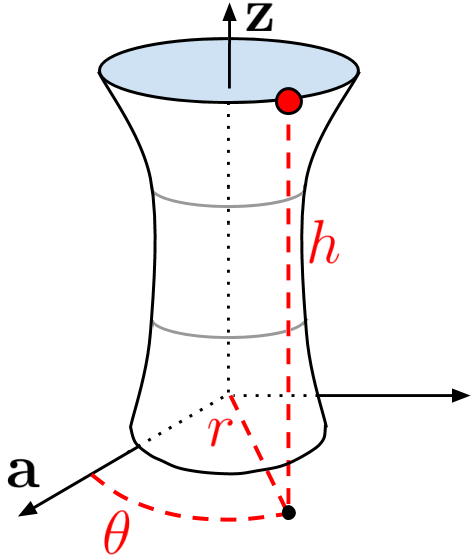
\includegraphics[width=0.75\linewidth]{./images/representation.png} \quad 
  \end{center}
  \caption{Cylindrical coordinate system to parameterize points on a rotationally symmetric object}
%   \caption{A of a
%   rotationally symmetric object. The axis $\vech{a}$ corresponds to the polar axis, while $\vech{h}$
%   is the axis of symmetry. Any point on the surface can be represented using height $h$, radius $r$,
%   and angle $\theta$. }
  \label{fig:representation}
\end{figure}

\newpage

A significant observation about the representation of rotationally symmetric objects in cylindrical
coordinates is the dependency of the radius $r$ and the height $h$ parameters. For a given shape $S$,
all the points on $S$, at some height $h$ along the principal axis $\vech{z}$, have the same distance
$r$ to the axis: $\forall p \in S$ s.t. $p \cdot \vech{z} = h$, $dist(p, \vech{z}) = r_S(h)$. The
function $r_S(h)$ represents the inherent curvature of the shape - for instance, for a cylinder, $r
= c$ for some constant $c$. Based on this observation, we can conclude that any contact point $p$ on
an object shape $S$ can in fact be parameterized minimally by two variables, $h$ and $\theta$.
In this work, we show that analyzing the task constraints, robot limitations and contact models 
in this low-dimensional subspace leads to significant efficiency gains in grasp planning.

%==================================================================================================
\subsubsection{Mapping Euclidean Coordinates to Reduced \\Cylindrical Space}

To reason about tasks traditionally expressed in Euclidean coordinates, we introduce a mapping 
between the representation of a point in the Euclidean world frame, $p_w$, to the $\vech{x} = [h,\theta]^T$
parameters in the reduced cylindrical space $\mathbb{S}$. First, we define the local object frame $L$ in the
Euclidean coordinate frames by using the principal axis $\vech{z}$, the polar axis $\vech{a}$, and
their cross-product. Given the pose of an object in the world coordinates, $T^w_l$, we can first
transform the point into the local object space, $p^l = T^l_w ~ p^w$, and then map it to the surface
representation $\vech{x}$ using the function $f: \mathbb{R}^3 \rightarrow \mathbb{S}$: 

% TODO Add [h \theta] to this equation?
\begin{equation}
  f(\vech{p}^l) = f([x,y,z]^T) = \left[ \begin{array}{c} z \\ atan2(y,x) \end{array}\right].
\end{equation}

Once a planner reasons about the environment and a contact point is determined in the cylindrical surface representation,
we need to map it back to the Euclidean space using an inverse mapping $f^{-1}: \mathbb{S} \rightarrow \mathbb{R}^3 $:

\begin{equation}
  f^{-1}(\vech{x}) = f^{-1}([h, \theta]^T) = \left[ 
  \begin{array}{c}
  r(h) ~ cos(\theta) \\ r(h) ~ sin(\theta)\\ h 
  \end{array} \right]. 
\end{equation}

Fig.~\ref{fig:unfolding} depicts the forward mapping process starting from the representation of
a contact point in the world coordinate frame, moving to the local object frame and finally transformed
to the cylindrical surface representation. Observe that the surface of the example soda can be unwrapped
into a smooth finite two-dimensional plane with minimal distortion because the object is rotationally
symmetric, and does not have protrusions nor cavities. 

\begin{figure}[ht!]
  \begin{center}
    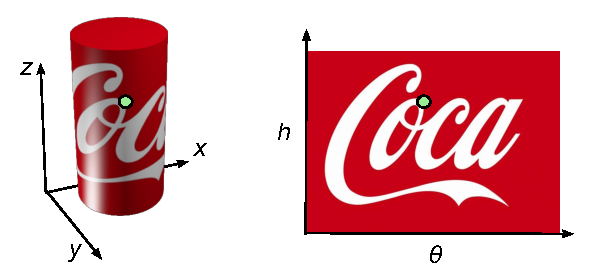
\includegraphics[width=0.45\textwidth]{./images/unfolding.pdf} \quad
  \end{center}
  \caption{The points on the 3D surface (left) are projected onto a 2D cylindrical manifold.}
  \label{fig:unfolding} 
\end{figure}

%==================================================================================================
\subsection{Grasp Manifold}

\textit{Stable grasps can be rotated around the principle axis of rotationally symmetric objects
without having to modify the hand shape}. Moreover, the relative rotation between a predefined grasp
and an object can be captured with a simple linear motion model in the reduced 2D cylindrical
manifold. To demonstrate the advantages of these key ideas, we begin our analysis with a simplified
manipulation model where a point on the object surface corresponds to a wrist position during
grasping. Moreover, the hand is assumed to be parallel to the base of the object such that the plane
between the grasping fingers is perpendicular to the axis of symmetry. 

Given a predefined hand shape and a task definition, the planner needs to choose a contact point,
$\vech{x} = [h, \theta]$, that represents its wrist position. Feasible contact points are characterized
by collision-free inverse kinematic solutions where at least one manipulator pose should exist that 
both reaches the desired point and does not collide with the environment. In addition to the physical
feasibility of a contact point, its functionality towards accomplishing tasks also needs to be
taken into account in grasp selection. For instance, if an object is picked with the purpose of
placing it down in another cluttered environment, collisions in the second scene also need to be
accounted for. Similarly, a task may require an object to be configured at a specific pose, i.e.
pouring water from a bottle to a cup, in which case the planner should account for the reachability of
that pose with the \textit{foresight} that the same grasp would have to be utilized. 

%==================================================================================================
\subsubsection{Modeling Task Constraints in Cylindrical Space}

Most everyday grasps require reasoning about multiple tasks even though the tasks may take place in
substantially different environments with varying constraints on the pose of the manipulated
object. Although the locations and requirements of the tasks may vary, they all impose constraints 
on the same gripper-object system since once an object is picked, the grasp cannot be changed. 
We exploit the \textit{invariance} of the gripper-object relationship in manipulation tasks with 
rotationally symmetric objects, where the task descriptions naturally account for all the degrees 
of freedom but the rotation around axis of symmetry since the rotation does not effect object
properties. The goal is to autonomously exploit the under-constrained task specifications by
planning for object rotations and grasp positions. 

By only modeling grasps that are perpendicular to the axis of symmetry, e.g. grasp
rotates around object, we induce a coupling between gripper and object poses. Now, \textit{given a
single pair of gripper and object poses that is known to satisfy task constraints, an infinite
number of new pairs can be generated by rotating the gripper around the object by some $\theta$ degrees and rotating the object
around itself by $-\theta$}. Moreover, by determining the feasible set of contacts for an initial object
pose which satisfies task requirements, we can extrapolate to a family of object rotations
and corresponding contact placements. This extrapolation is only feasible because the rotation
of the object around its axis and the rotation of the grasp around the object are coupled by 
the $\theta$ variable around the principle axis $\vech{z}$ and thus, we reason about task
constraints in the cylindrical parameter space.

The idea is as follows. For each task.... 
To sample this space, we propose discretizing the manifold by fixed
step sizes for the height $h$ and the angle $\theta$. Refer to picture. For each patch of the
discretized manifold, using the center point  as the reference for the wrist, we attempt to compute
a collision-free inverse kinematics solution. Refer to picture again showing red/blue and which
collisions were caused. 

\begin{figure}[ht!]
  \begin{center}
    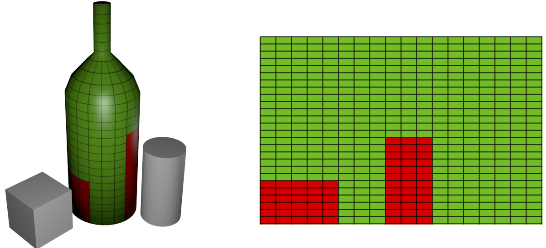
\includegraphics[width=0.45\textwidth]{./images/bottlemapping.png} \quad
  \end{center}
  \caption{The points on the 3D surface (left) are projected onto a 2D cylindrical manifold.}
  \label{fig:unfolding} 
\end{figure}


A crucial property of this representation is that the produced map can
be efficiently updated when the object is rotated around its axis of symmetry. More specifically, a
rotation around the z-axis corresponds to a shift along the $\theta$ dimension. 

\begin{figure*}[t]
  \begin{center}
    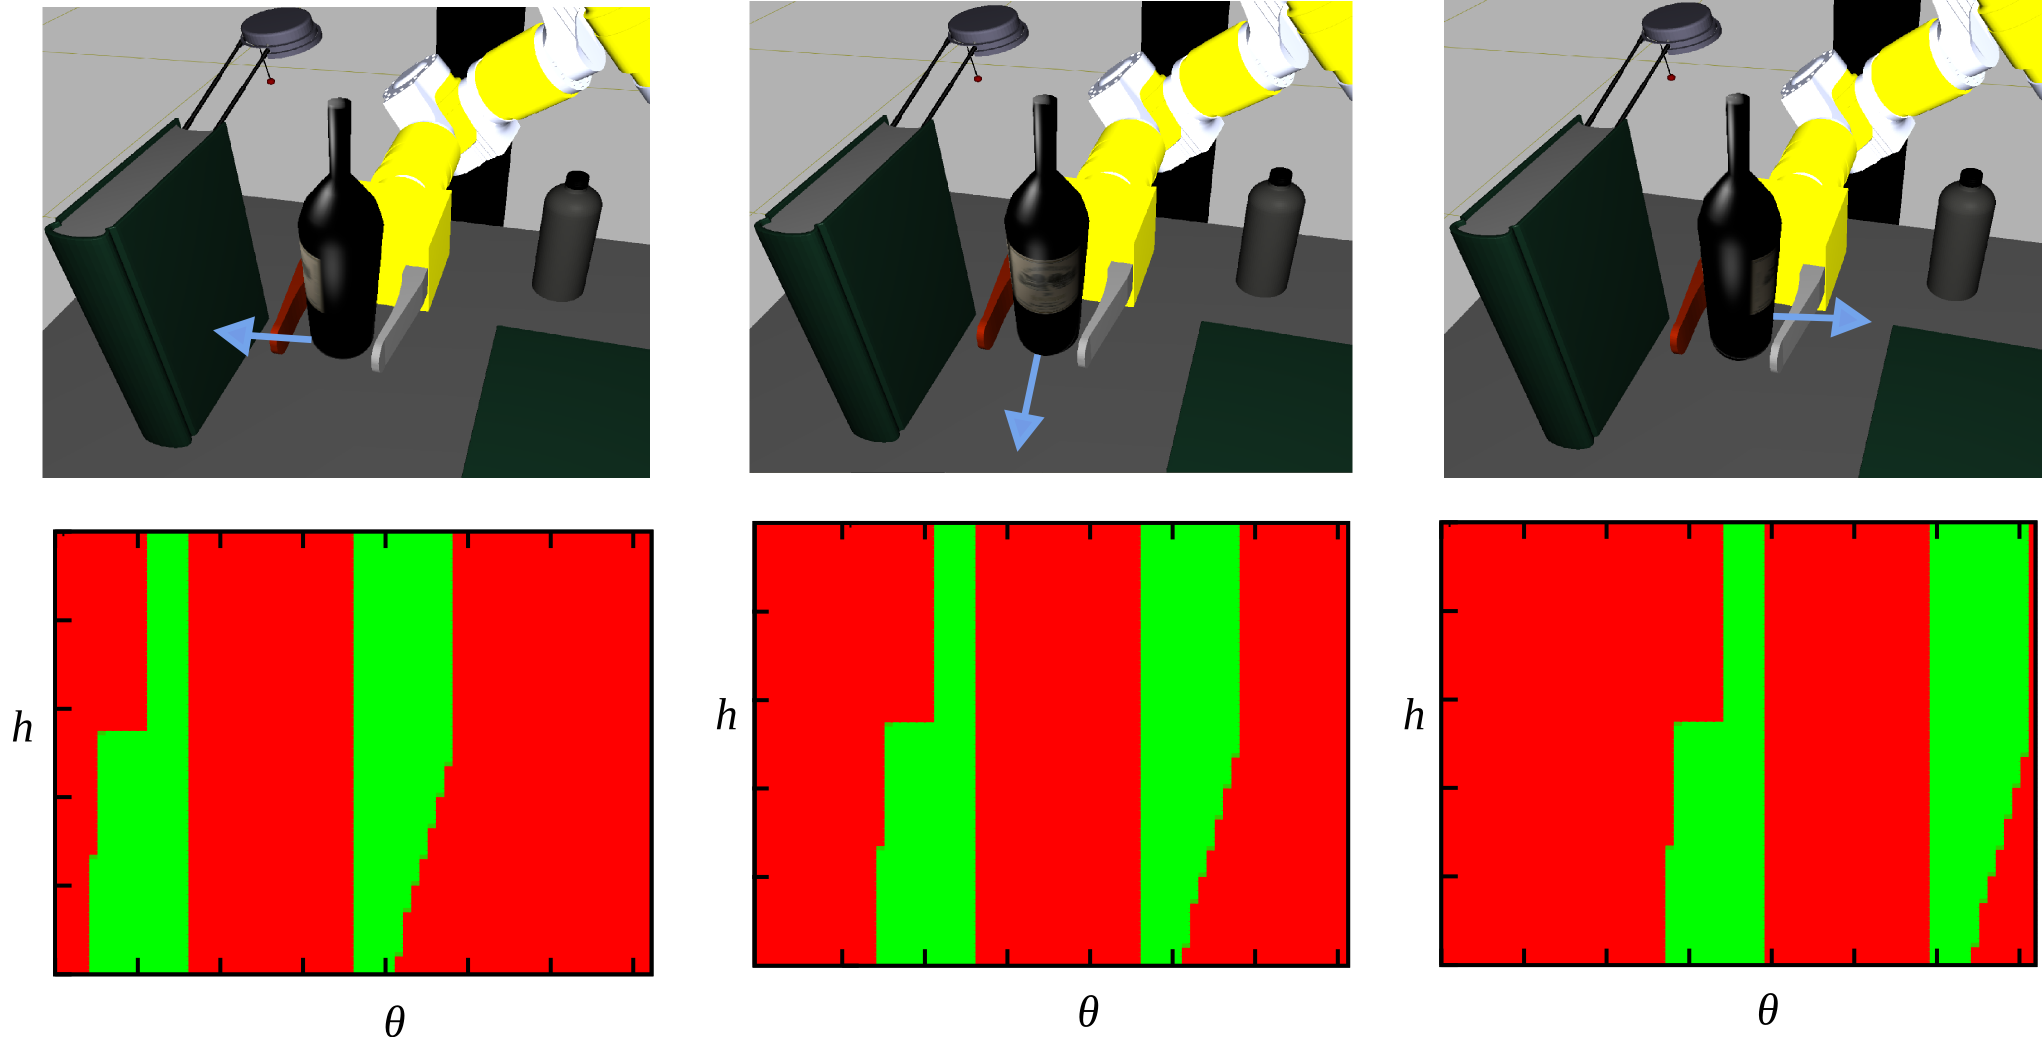
\includegraphics[width=0.75\linewidth]{./images/rotatingWine.png} \quad
  \end{center}
%   \caption{The points on the 3D surface (left) are projected onto a 2D cylindrical manifold.}
  \label{fig:unfolding} 
\end{figure*}

%==================================================================================================
\newpage
\subsubsection{Extrapolating task constraints to different \\object rotations}

The analysis of grasp feasibility for a given object pose and task description can be utilized to reason
about grasp selection if the object is rotated only around its axis of symmetry. The idea is that the 
coupling between the rotation of the grasp around the object pose and the rotation of the object around
its own principle axis can be utilized to generate previously examined grasps for new object rotations
and to adopt the successful examples. The invariance of task constraint effects on gripper-object
systems to interactions between the gripper and the object poses that do not change gripper configuration
in the task space can be analyzed formally. 

Let the function $m: \mathbb{S}, SE(3) \rightarrow \{0,1\}$ represent a mapping from a 6-DOF object
pose $T^w \in SE(3)$ and a contact pose on the object surface, $\vech{x} = [h, \theta]^T \in \mathbb{S}$,
to a binary evaluation of whether a grasp is feasible. The feasibility of a grasp may depend on a variety
of criteria such as inverse kinematics, collisions, torque limits, manipulability and etc. In this work,
we focus on collision-free inverse kinematics and define the operator $ik: SE(3) \rightarrow \{0,1\}$
that evaluates whether an arm configuration exists that can achieve the end-effector pose $T^w_e \in SE(3)$. 

We claim that given the mapping of feasibility grasps for an initial object pose $T^w_o$, the feasibility of any 
grasp $x \in \mathbb{S}$, for a new pose $T^w_{o_2}$, can be deduced by using the previous mapping:

\begin{equation}
  m([h,\theta],T^w_{o_2}) = m([h,\theta+\delta], T^w_o)
\end{equation}

\noindent where $T^w_{o_2} = T^w_o ~ R^z(\delta)$ where $R^z$ is a rotation matrix around the local $z-axis$




































%==================================================================================================
% cyclic manifold 
% \begin{enumerate}
%   \item Define frames $L$ and $G$ as local object frame and global frame
%   \begin{enumerate}
%     \item 
%     Let $\vech{z}$ be the axis of symmetry, $\vech{o}$ be the origin, and $\vech{a}$ be the polar axis of the object.The polar axis lies in the reference plane of the object and is perpendicular to $\vech{z}$. In the following, we assume that the reference plane is the base of object. Note that $\vech{a}$ can be arbitrarily chosen, since the object is symmetric. Using $\vech{z}$, $\vech{a}$ and their crossproduct we can form a local coordinate frame $L$ for an object.
%     
%     \item Any point $\vech{p} = [x,y,z]^T$ in the local coordinate frame $L$, can also be represented using a cylindrical parametrization of the coordinate system. 
%     
%     \item This parametrization leads to a point $[h, r, \theta]^T$ whose components correspond to the height, radius and angle respectively. The height is measured along the axis of symmetry $\vech{z}$, the radius $r$ is the distance between $\vech{p}$ and $\vech{z}$, the angle $\theta$ is the angle between $\vech{a}$ and the projection of $\vech{p} $ onto the local reference plane of the object as can be seen in Fig.~\ref{}. 
%     
%     \item In the following, we define the radius as a function $r(h)$ of the height, which leads to a two-dimensional parametrization $[h, \theta] \in \mathbb{S}$ of point $\vec{p}$. Subsequently, we can define the function $f: \mathbb{S} \rightarrow \mathbb{R}^3$ that maps the cylindrical coordinates to the 3D local coordinates in the following way:
%     
%     \begin{equation}
% 	    f(\vech{x}) = f([h, \theta]) = [r(h) ~ cos(\theta), r(h) ~ sin(\theta), h]
%     \end{equation}
%     
%     \item Similarly, we can map from the 3D local coordinate space $L$ to the 
%     surface manifold using the inverse mapping, $f^{-1}: \mathbb{R}^3 \rightarrow \mathbb{S}$:
%     
%     \begin{equation}
% 	    f^{-1}(\vech{p}) = f^{-1}([x,y,z]) = [z, atan2(y,x)]
%     \end{equation}
%   
%     \item Wrap up: Having defined the forward and backward mappings, now we can discuss how this is useful.
%   \end{enumerate}
	
% 	\item Parametrizing Grasps using Low Dimensional Manifolds
% 	\begin{enumerate}
% 		
% 		\item In this section, we demonstrate how to exploit the introduced representation and the symmetry properties of the object to efficiently sample feasible grasps. The key insight is that stable grasps can be rotated around the axis of symmetry without having to modify the hand shape. 
% 			
% 		\item We begin the analysis with a simplified grasping model where a point
% 		on the surface corresponds wrist position during grasping. The hand is assumed to be parallel to the base of the object such that the plane between the grasping fingers is perpendicular to the axis of symmetry. 
% 
% 		\item The goal is to identify the set of feasible points the robot can grasp. This requires reasoning about reachability and collisions, where we need to ensure that there is a collision-free arm pose with the wrist touching the respective surface point. To sample this space, we propose discretizing the manifold by fixed step sizes for the height $h$ and the angle $\theta$. Refer to picture.
% 		
% 		\item For each patch of the discretized manifold, using the center point 
% 		as the reference for the wrist, we attempt to compute a collision-free 		inverse kinematics solution. Refer to picture again showing red/blue and which collisions were caused. 
% 		
% 		\item An interesting property of this representation is that the produced map can be efficiently updated when the object is rotated around its axis of symmetry. More specifically, a rotation around the z-axis corresponds to a shift along the $\theta$ dimension. 
% 		
% 		\item 
% 	\end{enumerate}
	
% 	\item Low-dimensional manifold for grasps on symmetric objects	
% 	\begin{enumerate}
% 	\item Let $\vech{x} \in \set{S}, where \vech{x} = [h, \theta]^T$
% 	\item $h$ is the height of the contact point along the axis of symmetry
% 	\item $r$
% 	\end{enumerate}

% \end{enumerate}

% name it!
% unwrapping introduces a nonlinear warping
%

% symmetry and invariance
% Pic1: wiki cylinder parameterization
% Pic2: coke picture
% Pic3: discretization and red/blue stuff with bottle
% Pic4: multiple hand rotations around object (wine bottle)
% Pic5: project robotiq hand onto coke

\newpage
\section{Task Planning with Grasp Manifolds}
% Pic5: two tasks superimposed on top of each other (manifold pictures and simulation) and one object rotating

\newpage 
\subsection{Planning for Task Sequences}
% Pic6: Rod through 3 tasks (superimposed)

\newpage
\subsection{Planning for Bi-Manual and Cooperative Tasks}
% Pic7: Hand prints of two robots (two different robot hands, robotiq vs. tweezer)
% Pic8: Picture of two robots in front of each other, hand over

\newpage
\section{Experiments}
% offline experiment: how fast is map generation? 
% online experiment: how fast is sequence generation?
% quality? how good? alternative solutions?
% Pic8: 3D blob
% 2 different domains
 
 \newpage
\section{Discussion}
% this representation introduces warping effects
% talk about variable radius objects (picture)
% hierarchical grid, importance, details lost
% using profile instead of height
\newpage
\section{Conclusions}

\end{document}
